\chapter{Grundlagen}
Dieses Kapitel verschafft einen Überblick über die benötigten theoretische Grundlagen, um die Methoden dieser Arbeit zu verstehen. Als
erstes wird der ``Lab-Farbraum'' kurz erklärt. Als nächstes wird eine Einführung in Neuronale Netzwerke gegeben, anschließend werden
einzelne Bestandsteile und Varianten von Neuronalen Netzwerken erklärt. Abschließend wird einen Überblick über verwandte Arbeiten gegeben.

\section{\textit{Lab}-Farbraum} 
Der \textit{Lab}-Farbraum (auch CIELAB-Farbraum genannt) ist ein Farbraum definiert bei der Internationale
Beleuchtungskommission (\gls{cie}) in 1976. Farben werden mit drei Werte beschrieben. ``\textit{L}'' (Lightness) definiert die Helligkeit.
Die Werte liegen zwischen 0 und 100. ``\textit{a}'' gibt die Farbart und Farbintensität zwischen Grün und Rot und ``\textit{b}'' gibt die
Farbart und Farbintensität zwischen Blau und Gelb. Die Werte für ``\textit{a}'' und ``\textit{b}'' liegen zwischen -128 und 127.

TODO: image
% TODO: add color space image
% \begin{figure}[H]
%   \centering
%   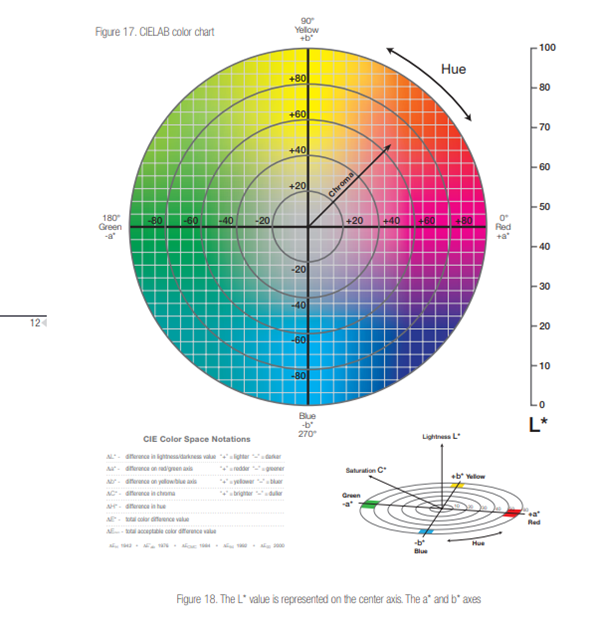
\includegraphics[width=0.5\textwidth]{resources/colorspace/lab-color-space.png}
%   \caption{CIELAB Farbraum}
%   \label{}
% \end{figure}

\section{Neuronale Netze}
Künstliche Neuronale Netze sind inspiriert durch das Menschliche Gehirn und werden für Künstliche Intelligenz und Maschinelles Lernen
angewendet. Sie werden für überwachtes und unüberwachtes lernen verwendet. In der vorliegende Arbeit werden nur Methoden des überwachtes 
lernen angewendet. Bei überwachtes lernen sind die Datensätze gelabelt sodass den Output von dem Neuronales Netz mit den richtigen Ergebnissen
verglichen werden kann.
\\
\\
Neuronale Netze bestehen aus Neuronen oder auch ``Units'' genannt, die Schichtenweise in ``Layers'' (Schichten) angeordnet sind.
Beginnend mit der Eingabeschicht (Input \gls{Layer}) fließen Informationen über eine oder mehrere Zwischenschichten (Hidden \gls{Layer}) bis hin zur 
Ausgabeschicht (Output \gls{Layer}). Dabei ist der Output des einen Neurons der Input des nächsten. \cite{neuronale-netze-aufbau}

\subsection{Feedforward Neural Network}
Das Ziel von einem Feedforward Neural Network ist die Annäherung an irgendeine Funktion $ f^* $. Ein Feedforward Neural Network definiert 
eine Abbildung $ y = f(x;\theta) $ wo $ x $ den Input ist und $ \theta $ die lernbare Parameter sind (auch Weights genannt).
\cite[164-223]{Goodfellow-et-al-2016}
\\
\\
Diese Netzwerkarchitektur heißt ``feedforward'' weil der Informationsfluss von der Input \gls{Layer} über die Hidden Layers bis zur Output \gls{Layer} 
in einer Richtung weitergereicht wird.

Feedforward Neural Networks werden als eine Kette von Funktionen repräsentiert. Als Beispiel,
kann man die Funktionen $ f^{(1)}, f^{(2)}, f^{(3)} $ in Form einer Kette verbinden um $ f(\textbf{x}) = f^{(3)}(f^{(2)}(f^{(1)}(\textbf{x}))) $
zu bekommen. Diese Kettenstrukturen sind die am häufigsten genutzte Struktur bei Neuronale Netzwerke. In diesem Fall, $ f^{(1)} $ ist das 
erste Layer, $ f^{(2)} $ das zweite und $ f^{(3)} $ der Output Layer von diesem Netzwerk. Die Länge dieser Kette definiert die Tiefe von
einem Netzwerk. Je tiefer
ein Netzwerk ist desto mehr lernbare Parameter hat es und somit eine erhöhte Rechenleistung braucht um trainiert zu werden.
In der Praxis werden die Netzwerke sehr tief, daher der Begriff Deep Learning.
\\
\\
Während dem Training werden die Weights von $ f(x) $ verstellt, um $ f^*(x) $ zu erhalten. Jedes Trainingsbeispiel $ x $ ist mit einem Label
$ y = f^*(x)$ versehen. Die Trainingsbeispiele legen genau fest, was der Output Layer generieren soll. Der Output Layer soll Werte generieren,
die nah an $ y $ liegen. Das Verhalten von den Hidden Layers wird nicht durch die Trainingsbeispiele festgelegt, sondern der Lernalgorithmus
soll definieren, wie diese Layers verwendet werden, um die beste Annäherung von $ f^*(x) $ zu generieren. \cite[164-223]{Goodfellow-et-al-2016}

\subsection{Fully-connected Neural Network}
Fully-connected Neural Networks sind die am häufigsten vorkommende Art von Neuronale Netze. In dieser Netzwerkarchitektur sind alle Neuronen
von einem Layer mit alle Neuronen von der vorherige und nächsten Layer verbunden. Neuronen in dem gleichen Layer sind aber nicht miteinander verbunden.
\cite{cs231-neural-networks}

\begin{figure}[H]
  \centering
  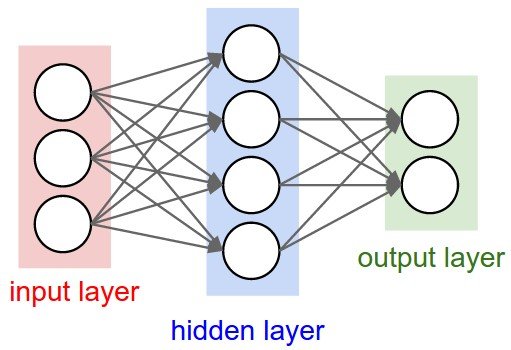
\includegraphics[width=0.65\textwidth]{resources/nn/neural_net.jpeg}
  \caption{
    Fully-connected Neural Network mit 2 Layers (ein Hidden Layer mit 4 Neuronen) und ein Output Layer mit 2 Neuronen 
    \cite{fully-connected-neural-network}
  }
  \label{image:neuronal-network}
\end{figure}

Eine der wichtigsten Gründe für die Anordnung von Neuronale Netze in Layers ist dass so eine Struktur anhand von Matrix Multiplikationen
berechnet werden kann. Das obere Bild \ref{image:neuronal-network} stellt ein Netzwerk mit 3 Inputs $ x $, eine Hidden Layer mit 4 Neuronen
und eine Output Layer mit 2
Neuronen dar. Die Kreisen repräsentieren die Neuronen und einem Bias Wert $ b $, die Pfeilen stellen die Weights $ w $ dar.

\begin{align}
  f(x) = w*x + b
\end{align}

Nach jeden Hidden Layer läuft den Output durch eine Aktivierungsfunktion $ \sigma $ die in \ref{subsection:aktivierungsfunktionen} erklärt wird.
Daraus wird die vorherige Formel um $ \sigma $ erweitert:

\begin{align}
  f(x) = \sigma( w*x + b)
\end{align}

\subsubsection{Forward Pass}
Den Forward Pass von einem Neuronalem Netz wird anhand von Matrizen Multiplikationen berechnet. Um das zu veranschaulichen wird
es anhand eines Beispiels erklärt.

Ausgehend von einem Netzwerk mit 3 Inputs, eine Hidden Layer mit 2 Neuronen und einem Output Neuron, ergeben sich folgende Beispielwerte:
\begin{equation} 
  \vspace{5pt}
  X = \begin{pmatrix}
    1 &0 &1 &1 \\
    1 &1 &1 &0 \\
    1 &1 &0 &1
  \end{pmatrix} 
  \hspace{5pt}
  W = \begin{pmatrix}
    10 &20 \\
    -20 &-40 \\
    20 &0 \\
    -40 &0
  \end{pmatrix}
  \hspace{5pt}
  W_{out} = \begin{pmatrix}
    20 \\
    40 \\
    -40
  \end{pmatrix}
\end{equation}

Die erste Spalte in der Input Matrix $ X $ und die erste Zeile in beide Gewichtsmatrizen $ W $ und $ W_{out} $ sind die Werte für den Bias.
Diese Anordnung von den Bias Werte ermöglicht die Berechnung durch eine einzigen Matrix Multiplikation. Als Aktivierungsfunktion wird ReLU\cite{10.5555/3104322.3104425} verwendet:

\begin{equation}
  \vspace{5pt}
  \sigma(x) = 
  \begin{cases}
    0 &\text{if \(x < 0\)}  \\
    x &\text{if \(x \geq 0\)} 
  \end{cases}
\end{equation}

Im ersten Schritt durchläuft den Input durch das Hidden Layer $ \sigma(X \times W) $:
\begin{equation}
  \vspace{5pt}
  \sigma \left(
  \begin{pmatrix}
    1 &0 &1 &1 \\
    1 &1 &1 &0 \\
    1 &1 &0 &1
  \end{pmatrix}
  \times
  \begin{pmatrix}
    10 &20 \\
    -20 &-40 \\
    20 &0 \\
    -40 &0
  \end{pmatrix}
  \right)
  =
  \begin{pmatrix}
    0 &1 \\
    1 &0 \\
    0 &0
  \end{pmatrix}
\end{equation}

Im zweiten Schritt wird den Output von der vorherige Multiplikation mal die Gewichte von dem Output Layer multipliziert:
\begin{equation}
  \vspace{5pt}
  \sigma \left(
  \begin{pmatrix}
    1 &0 &1 \\
    1 &1 &0 \\
    1 &0 &0
  \end{pmatrix}
  \times
  \begin{pmatrix}
    20 \\
    40 \\
    -40
  \end{pmatrix}
  \right)
  =
  \begin{pmatrix}
    0 \\
    1 \\
    0
  \end{pmatrix}
\end{equation}

% \begin{figure}[H]
%   \centering
%   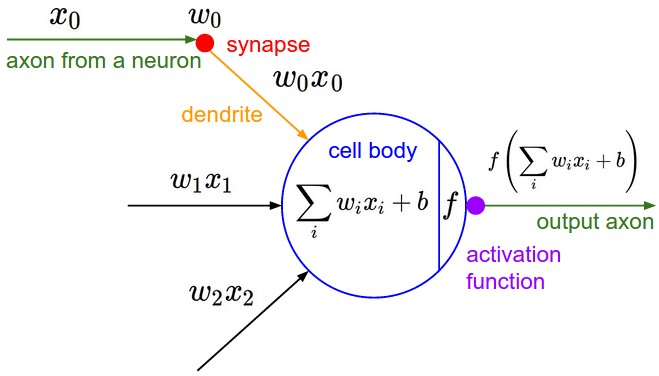
\includegraphics[width=0.65\textwidth]{resources/nn/neuron_model.jpeg}
%   \caption{
%     Mathematisches Model eines Neurons 
%     \cite{neuron-model}
%   }
%   \label{image:neuron-model}
% \end{figure}

\subsection{Aktivierungsfunktionen}\label{subsection:aktivierungsfunktionen}
Eine Aktivierungsfunktion definiert die Aktivierungsrate von einem Neuron. Es gibt verschiedene Aktivierungsfunktionen:

\subsubsection{Sigmoid}
Sigmoid ist eine nicht lineare Funktion $ \sigma(x) = 1 / (1 + e^{-x})$ welche die Werte in einem Wertebereich von $ [0, 1] $ bringt.


\subsubsection{Tanh}

\subsubsection{ReLU}
Die Rectified Linear Unit berechnet $ f(x) = max(0, x) $, alle negative Werte werden 0 und alle positive Werte bleiben gleich.

\begin{figure}[H]
  \centering
  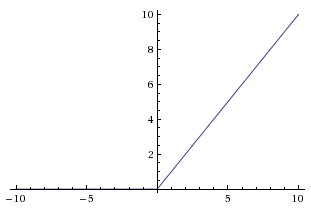
\includegraphics[width=0.65\textwidth]{resources/nn/relu.jpeg}
  \caption{
    Rectified Linear Unit (ReLU) 
    \cite{neuron-model}
  }
  \label{image:relu}
\end{figure}

\subsection{Convolutional Neural Network}
\subsection{Kostenfunktionen}
\subsection{Backpropagation}\label{subsection:backpropagation}
\subsection{Optimierungsalgorithmen}
\subsection{Max Pooling Layer}
\subsection{Transposed Convolution}
\section{Verwandte Arbeiten}
TODO